
\section{Grundlagen}
\subsection{Was ist Python?} %TODO ADD INFORMATION AND INTRODUCTION
Die Programmiersprache Python wurde Anfang der 1990er Jahre von Guido van Rossum entwickelt.
Der Name der Sprache beruht auf der Komikergruppe  Monty Python.
Hierzu lassen sich auch zahlreiche Anspielung in der Dokumentation von Python finden.
Python wurde mit dem Ziel gr��ter Einfachheit sowie �bersichtlichkeit entworfen.
Dies wird nicht zuletzt durch die gr��e �bersichtlichkeit in der Standardbibliothek versucht zu erreichen sondern auch durch die Modulare Erweiterbarkeit.
Im folgenden wird die Python in der Version 3 behandelt.

\subsection{Installation}
Python kann auf der Webseite https://www.python.org bezogen werden.
Nach dem Download des Installationsassistenten kann dieser gestartet werden und f�hrt den Nutzer anschlie�end durch den Installationsprozess.
\subsubsection{Installation unter Windows}
%TODO Installation + Hinweis zur Pfad Variable
\subsubsection{Installation unter Mac}
Im Folgenden wird die Installation unter Mac OSX gezeigt.
Der Installationsprozess unterscheidet sich zwischen den Betriebssystemen nur gering bis gar nicht.

\begin{figure}[ht]
	\centering
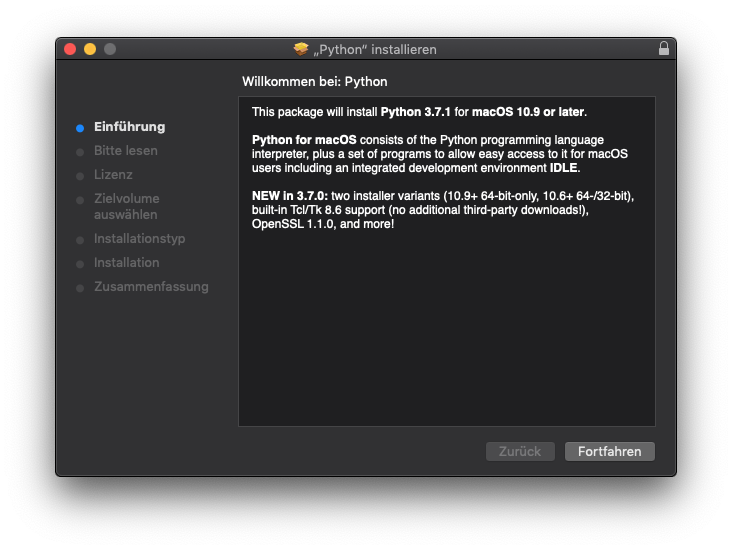
\includegraphics[scale=0.5]{images/Installationsassistent.png} 
	\caption{Start des Installationsassistenten}
	\label{fig:InstallAssist}
\end{figure}
Neben der Best�tigung der Lizenzvereinbarung muss w�hrend der Installation keine Auswahl getroffen werden.
Somit erscheint nach Ende der Installation der Python Ordner im Finder (Dateiexplorer).
\begin{figure}[ht]
	\centering
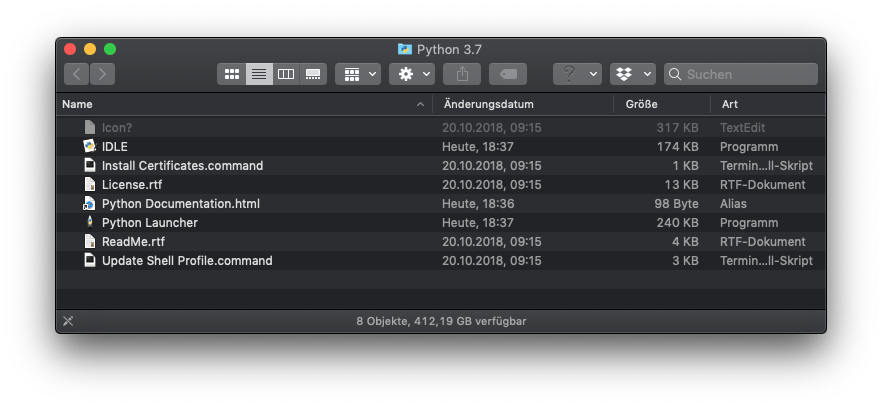
\includegraphics[scale=0.5]{images/PythonFinder.png} 
	\caption{Fertige Installation}
	\label{fig:FinishInstall}
\end{figure}
Nach Abschluss der Installation stehen dem Anwender die verschieden Programme zur Verf�gung.
Unter /Application/Python[Version] befindet sich \textit{IDLE}, die mitgelieferte Standard Entwicklungsumgebung zu Python.
Der \textit{PythonLauncher}, welcher f�r das ausf�hren von Python-Scripts per Doppelklick zust�ndig ist.
Das \textit{Build Applet} um Python Script zu lauff�higen Anwendungen zusammen zu packen.
Zuletzte wurde durch den Assistent unter /Library/Frameworks/Python.framework noch das Python Framework abgelegt.
Ohne dieses w�re das Arbeiten mit Python nicht m�glich.
%TODO Skript versus Programm

\subsection{Python Interpreter} %WIP ROGU 
%TODO ADD LINKS TO OTHER SECTIONS %WHAT IS PYTHON CODE?
Die einfachste M�glichkeit, Python Code auszuf�hren, ist direkte �bergabe des Codes an den sogenannten Python Interpreter. 
Dabei handelt es sich um eine Konsolenanwendung, welche Code ausf�hrt und gegebenenfalls Ergebnisse ausgibt. 
Dabei kann ein Nutzer den Code entweder direkt in die Konsole eingeben oder diesen aus einer Datei auslesen lassen. 
Wie bei anderen Programmiersprachen auch, stehen verschiedene IDEs\footnote{Integrated Development Environment} zur Verf�gung, welche in Kapitel \ref{} behandelt werden. 
F�r die ersten Versuche mit Python reicht der Interpreter jedoch v�llig aus. Dieser wird standardm��ig mit Python installiert.\\
In Abbildung \ref{fig:Interpreter} ist der Interpreter zu sehen. 
Zus�tzlich zur Version werden auch noch der Herausgeber von Python sowie die Uhrzeit angezeigt.
Bereits jetzt kann erster Code ausgef�hrt werden.
Im Folgenden werden zu einzelnen Bestandteilen von Python Beispiele beigef�gt, welche leicht im Interpreter ausf�hrbar sind. Es wird dem Leser empfohlen, diese zum besseren Verst�ndnis nachzuvollziehen, falls m�glich durch eigenst�ndiges Ausprobieren.
\begin{figure}[ht]
	\centering
	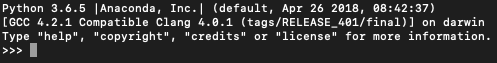
\includegraphics[width=0.8\textwidth]{images/Interpreter.png} 
	\caption{Ansicht nach Start des Interpreters}
	\label{fig:Interpreter}
\end{figure}
 
\paragraph{Interaktiver Modus} 
Wird der Interpreter ohne Angabe einer Quellcodedatei gestartet, befindet dieser sich im interaktiven Modus. 
Der Nutzer kann hier direkt Anweisungen eingeben. Durch die Ausgabe der Zeichen ''>>>'' zeigt die Konsole an, dass sie eine Anweisung erwartet. 
In Python existieren auch mehrzeilige Anweisungen. 
Nach der Eingabe der ersten Zeile, werden die Zeichen ''...'' ausgegeben, was bedeutet, dass Folgeanweisungen erwartet werden. 
\paragraph{Einlesen einer Datei} %WIP ROGU
Dateien, welche Python Code enthalten werden mit der Dateiendung ''.py'' gekennzeichnet. 
Sie k�nnen direkt mit dem der Konsole ausgef�hrt werden.
Dazu muss der ausf�hrbaren Datei ''python.exe'' der Pfad der Python-Datei �bergeben werden. 
\subsection{Syntax}
Folgende syntaktische Besonderheiten Bringt Python mit:
\subsubsection{Ausdr�cke} %WIP ROGU
Anders als bei anderen Programmiersprachen wie beispielsweise Java, ben�tigt Python keine Klassenkonstrukte... %TODO AUSDRÜCKE, kein fester Rahmen zur Ausführung benötigt
\subsubsection{Einfache Datentypen}
\subsubsection{Leerzeichen und Einr�ckung}
Um in Python Bl�cke auszuzeichnen k�nnen nicht wie in Java und C++ geschweifte Klammern genutzt werden. 
In Python ist hierf�r entweder der Tabulator oder 4 aufeinander folgende Leerzeichen vorgesehen.
Somit kann bei zum Beispiel einer IF-Abfrage der nachfolgende Block leicht falsch zugeordnet werden wenn in den nachfolgenden Zeilen die Einr�ckung �bersehen wird.
\subsubsection{Kommentare}
Innerhalb Python wird zwischen Zeilen und Blockkommentaren unterschieden.
Zeilenweise Kommentare werden �ber das Rautensymbol (\# ) eingeleitet.
Blockkommentare �ber drei aufeinander folgenden Anf�hrungzeichen ('''''').
Im folgenden jeweils ein Beispiel f�r Zeilenweise Kommentare sowie Blockkommentare.
\lstinputlisting{chapters/sections/listings/comment.py}
\subsubsection{Typsicherheit}
Anders als bei Java und C++ ist Python eine nur schwach typisierte Sprache.
Somit ist bei der Initialisierung keine Typangabe erforderlich. 
Der Datentyp wird beim Initialisieren dynamisch ermittelt und automatisch zugewiesen.
\subsubsection{Prozedurale Programmierung}
\subsection{Interpreter}
%übersetz das ihm übergebene Script
%kann als Umgebung genutzt werden


\subsection{Beispiel \glqq Hello World!\grqq}
Hier ein einfaches \glqq Hello World!\grqq -Beispiel.

\lstinputlisting{chapters/sections/listings/helloworld.py}
